\lab{Reinforcement Learning 1: Gymnasium}{Reinforcement Learning 1: Gymnasium}

\objective{Reinforcement learning is a topic found at the intersection between machine learning and control theory.
Gymnasium is a module designed to learn and apply reinforcement learning.
The purpose of this lab is to learn the variety of functionalities available in Gymnasium and to implement them in various environments to solve the reinforcement learning problem using trial and error and two model-free methods.}

\emph{Reinforcement learning}, or RL for short, is a problem, a class of solutions that work well on the problem, and a field that studies the problem and solutions to it.
As a problem, RL refers to the problem of getting an agent to explore an unknown environment to achieve a given task or goal.
That is, we have an agent in some world with a given objective it must accomplish in that world but the agent is not told what to do at any moment (i.e.\ the agent only knows that it can do some things).
You can think of this as baking a cake without a recipe and only being told you can open ingredients, mix them, and put them in the oven.
Thus, you know that you can mix, open, or bake eggs and flour, but you don't know if you first need to mix the eggs and flour together, then open them, and bake them or if it needs to be done in some other order.

As a class of solutions, RL refers to the various algorithms or computations whose tasks is to help an agent learn, through sequential decision-making and experience, how to interact with and learn from its environment in order to accomplish the given goal in the most optimal way possible.
It is different from other types of machine learning as reinforcement learning is concentrated more on goal-focused learning as a consequence of its interactions with the environment than other types of machine learning.
Thus, RL is the umbrella referring to the field of study encompassing all this.

We will introduce a summary of the theory behind reinforcement learning prior to the actual beginning of the lab.
Here are a few definitions to help you familiarize yourself with the verbiage used in RL (and by consequence in Gymnasium):
\begin{itemize}
    \item An \emph{agent}\footnote{In control theory, the agent is called the \emph{controller}, the environment is the \emph{plant} or \emph{controlled system}, and the action is the \emph{control signal}.} is a learner and decision maker whose goal is to learn a strategy or sequence of actions to accomplish a given task or goal.

    \item The \emph{environment} is the world in which the agent is located and consists of a set of different states.
    It is everything outside the control of the agent.

    \item The \emph{state}, denoted by $s$, is the set of information that describes the environment completely so as to enable the agent to take an action.
    Thus, a state is the current representation of the environment.
    The \emph{state space}, $S$, is the set of all possible states that the agent can be in, which includes the current state $s$ and all possible future states the agent can reach from $s$.

    \item An \emph{observation} is the information the agent gathers about the environment.
    Thus, the observation is the agent's perception or measurement of the state.
    In some cases, the observation may be a full measurement\footnote{In this case, the observation space is the state space so that the observation is equal to the state.} of the state, but in other cases, the observation is a partial representation of the state.

    \item The \emph{reward}, denoted by $r$\footnote{We talk more about the function case in the next RL lab.} or by a function $r(s^\prime,a,s)$ or $r(s,a)$ of states and actions, is a real scalar value used to define the goal the agent must accomplish.
    The reward is used to help the agent know, in the immediate sense, how good or bad the action or sequence of actions that it took was in helping it accomplish the goal.
    The set of all possible rewards that the agent can receive is denoted $\mathcal{R}$.

    \item A \emph{timestep} or \emph{time-period}, $t$, is the smallest discrete unit of time where the agent interacts with the environment once.
    This interaction typically comprises a cycle of one state, one action, and one reward.
    An \emph{episode} is a finite sequence of timesteps that starts at some \emph{initial state}, $s_0$ (i.e.\ the state at $t=0$), and ends at some \emph{terminal state}, $s_T$.
    The terminal state is the final state representing the end of an episode and can be a maximum number of timesteps or some other desired state.
    Note that in this latter case, the time of termination, $T$, can be different for each episode as well as the fact that each episode can have a different terminal state.
    When, we work with episodes, we call this the \emph{finite horizon}\footnote{When there an infinite amount of timesteps, we no longer use the word episode. We call this the \emph{infinite horizon} setting.} setting and use $S$ to denote the set of all non-terminal or normal states and $S^+$ to denote the set of all states, including the terminal states.
    We use $\mathbb{T}=\{0, 1,\ldots,T\}$ to denote the set of all time-steps, including the terminal time $T$, of one episode.

    \item A \emph{value function} returns the \emph{value} of a state or state-action pair as the expected future return of rewards.
    That is, the value function helps us determine the long-term desirability of a state or state-action pair after considering possible future states or state-action pairs that are likely to follow and the rewards that they will bring.
    Value functions estimate \emph{how good} it is for the agent to be in a given state or to take an action in a given state, after considering the expected future rewards.
    \begin{itemize}
        \item The \emph{state-action value}, \emph{quality of a state-action pair}, or \emph{action-value function} for a policy $\pi$, denoted by $q_\pi(s,a)$ or $q(s,a)$, is a function of state-action pairs that returns the value or \emph{quality} of a given pair as the expected return of taking action $a$ while being in state $s$ and following policy $\pi$ thereafter.
        In other words, given a state $s$, an action $a$, and a policy $\pi$ (i.e.\ a strategy to select an action based on a given state\footnote{We give a formal definition in the next RL lab.}), the value/quality of a state-action pair, $q(s,a)$, is the expected future return that the agent can receive by taking action $a$ while being in state $s$ at some period $t$ and enacting $\pi$ thereafter.
    \end{itemize}
\end{itemize}

\section*{The RL Interaction-Learning Framework}
In this section, we will assume that we are only working within one episode with a set $\mathbb{T}=\{0,1,\ldots,T\}$ of timesteps.

As mentioned earlier, in RL, the goal is to get an agent to learn, through sequential decision-making, how to interact with its environment in order to accomplish some given objective (e.g. teach a robot how to walk, a computer learning how to play chess, or have two chatbots generate dialogue etc.).
The agent interacts with the environment at each time-period $t\in\mathbb{T}$ by first receiving some observation of the current state $s$ of the environment at the that timestep $t$, denoted $s_t$.
Then based on this observation, the agent employs the mapping $\pi$ to select\footnote{In the stochastic/probabilistic case, the selection makes sense seeing there are multiple actions to choose from.
In the deterministic case, the selection is equal to performing the only action available. This will be covered in the next RL lab.} an action $a$ to perform for that time-period, denoted $a_t$.
One timestep later, $t+1$, the agent receives some feedback, a reward $r_{t}$, to help it know how good or bad the action $a_t$ was in helping it accomplish the task.
After this, the agent is now in the new state $s_{t+1}$ and the process begins again.
This same process of state, observation, action, and reward continues until we reach a terminal state\footnote{In the infinite horizon case, also known as \emph{continuous}, the process continues indefinitely.} and is one of the main aspects separating RL from other types of machine learning.
Note that the reward is received after the action is taken and when the agent is in a new timestep.
This is illustrated in Figure\ \ref{fig:RL_diagram}.

\begin{figure}[H]
    \centering
    \includegraphics[width=.7\textwidth]{figures/RLFramework.pdf}
    \caption{The reinforcement learning framework as given by \cite{sutton2018reinforcement}.
    Here, the reward is $R$ and $R_{t+1}$ is used to emphasize that the reward is received one time step later.
    Notice that the agent had received the reward $R_t$ for taking action $A_{t-1}$.
    This was given prior to choosing action $A_t$ during state $S_t$.
    The agent chooses the action $A_t$ based on the observation of $S_t$ and, to some extent, based on the reward $R_t$.
    The agent then goes to the next state $S_{t+1}$, receives the reward $R_{t+1}$, and the process repeats.}
    \label{fig:RL_diagram}
\end{figure}

Hence, the agent interacts with the environment by taking actions and receiving rewards.
These rewards are immediate feedback that the agent can use to determine how good an action is in helping it accomplish the task.
In some environments, the reward follows after each action, called \emph{dense rewards}, which can facilitate the problem.
In other environments, the reward may be \emph{sparsed} or delayed, perhaps until the end of the final timestep or until we fail/succeed, which makes the problem more challenging.

\section*{Reinforcement Learning Techniques}
The ultimate goal, that is the optimization problem, of RL is to learn an optimal policy, or optimal strategy to select actions based on given states, that will bring the agent the most future reward, which in turn helps the agent accomplish the given task.
There are several ways to solve the RL optimization problem.
The major division in RL techniques is between \emph{model-based} and \emph{model-free} methods.

In model-based methods, the agent has a model of the environment, which includes a model for any transitions between states as well as the rewards.
The agent makes use of this model to learn the optimal policy and updates the model as it interacts with the environment.
One goal can be to learn the dynamics of the environment and then use this to learn the optimal policy.
On the other hand, if we have certainty of the model and the dynamics, the agent can use this to evaluate future actions without having to try various actions and measuring the results of such actions as the model will help compute this.
In contrast, model-free methods do not have a model of the environment.
The agent learns by interacting with the environment and observing the rewards it receives rather than trying to learn the environment's dynamics or using a model to calculate future rewards.
Thus, the agent learns by trial and error and creates a policy based on the consequences of its actions.

\begin{figure}[H]
    \centering
    \includegraphics[width=.7\textwidth]{figures/RL_methods.pdf}
    \caption{A diagram of various techniques used to solve the reinforcement learning optimization problem as given by \cite{brunton2022data}.
    You can see this \href{https://www.youtube.com/watch?v=i7q8bISGwMQ&list=PLMrJAkhIeNNQe1JXNvaFvURxGY4gE9k74&index=4}{video} for a more in depth explanation.}
\end{figure}

The next RL lab, Reinforcement Learning 2: Markov Decision Process, is an example of a model-based method.
We will employ an MDP model on the environment and use the Bellman equations to find the optimal policy, assuming we know the dynamics of the environment.
In this lab, we will cover two model-free methods called \emph{Q-learning} and \emph{SARSA(0)}.
Thus, the main goal of this lab is to find the optimal policy through trial and error, without having a model of the environment.


\section*{Gymnasium Module}
Gymnasium is a module used to perform reinforcement learning.
It contains a collection of environments where reinforcement learning can be used to accomplish various tasks.
These environments include performing computer functions such as copy and paste, playing Atari video games, and controlling robots.
To install Gymnasium, simply run the following code:
\begin{lstlisting}
>>> pip install gymnasium
>>> # You may also need to install these dependencies
>>> pip install gymnasium[all]
>>> pip install gymnasium[classic-control]
\end{lstlisting}

\subsection*{Environments}

Each environment in Gymnasium can be thought of as a different scenario where reinforcement learning can be applied.
A catalog of environments can be found using the following code.

\begin{lstlisting}
>>> from gymnasium import envs
>>> print(envs.registry.values())
dict_values([EnvSpec(id='CartPole-v0', entry_point='gymnasium.envs.classic_control.cartpole:CartPoleEnv', reward_threshold=195.0, nondeterministic=False, max_episode_steps=200, order_enforce=True, autoreset=False, disable_env_checker=False, apply_api_compatibility=False, kwargs={}, namespace=None, name='CartPole', version=0, additional_wrappers=(), vector_entry_point='gymnasium.envs.classic_control.cartpole:CartPoleVectorEnv'), ...
\end{lstlisting}
To learn more about Gymnasium and its environments, visit \url{gymnasium.farama.org}.

We will demonstrate how to work with Gymnasium environments by walking through the environment \li{"Blackjack-v1"}.
The game Blackjack\footnote{For more on how to play Blackjack, see \url{https://en.wikipedia.org/wiki/Blackjack}.} is a card game where the player receives two cards from a face card deck.
The goal of the player is to get cards whose sum is as close to 21 as possible without exceeding 21.
In this version of Blackjack, an ace is considered 1 or 11 and any face card is considered 10.
On each turn, the player may choose to take another card or stop drawing cards.
If their card sum does not exceed 21, they may take another card, but if it does, they lose.
After the player stops drawing cards, the computer may play the same game.
If the computer gets closer to 21 than the player (without exceeding 21), the player loses.

To begin working in an environment, the environment must be initialized and reset.
Resetting the environment puts everything in the correct starting position and is necessary to begin using the environment.
For example, in \li{"Blackjack-v1"}, restarting the environment deals out a new game of Blackjack.
Once the environment is complete, it should then be closed.
Closing the environment tells the computer to stop running the environment (otherwise it will continue to run in the background).

\begin{lstlisting}
>>> import gymnasium as gym
>>> env = gym.make('Blackjack-v1')  # Initialize Blackjack-v1 environment
>>> env.reset()  # Reset the environment
((16, 6, 1), {})

>>> env.close()  # Close the environment
\end{lstlisting}

\subsection*{Action Space}
An \emph{action}, denoted by $a$, is the decision that the agent makes, while being in some state $s$, on what to do next.
The set of all possible actions that the agent can enact during some state $s$ is called the \emph{action set} or \emph{set of allowable actions}, denoted by $A_s$.
The overall set of all possible actions that the agent can take is denoted $A=\cup_{s\in S} A_s$ and is called the \emph{action space}.
Note each state\footnote{This does imply that all action spaces of terminal states are empty since the episode has finished. This does not mean you cannot get a reward at any terminal state.} $s\in S$ has an associated $A_s$.

Once the environment is initialized and reset, the player can perform actions from the action space.
To perform an action, use the function \li{step()}, which accepts the action as a parameter and returns an observation (more on those later).
Environments may have discrete or continuous action spaces, but the environments presented in this lab all have discrete action spaces.
When the action space is discrete, actions are defined as integers 0 through $n$, where $n$ is the number of actions.
The action each integer represents can be found in the documentation of each environment.
The action space in \li{"Blackjack-v1"}\footnote{The documentation can be found \href{https://gymnasium.farama.org/environments/toy_text/blackjack/}{here}} has 2 actions, represented by 0 and 1: 0 indicates that the player will stop drawing cards, and 1 indicates that the player will draw another card.

\begin{lstlisting}
>>> env = gym.make('Blackjack-v1')
>>> env.reset() # Returns the initial state
((12,9,0),{})
>>> env.action_space  # Determine the number of actions available
Discrete(2)
# Select a random action and take a step using that action
>>> random_action = env.action_space.sample()
>>> random_action
1
# In this case, the random action was to draw another card
>>> env.step(random_action)
((16, 9, 0), 0.0, False, False, {})
\end{lstlisting}

\subsection*{Observation Space}
The \emph{observation space} of an environment contains all possible observations.
For example, in \\ \li{"Blackjack-v1"}, an observation is a tuple containing the total sum of the player's hand, the first card of the computer's hand, and a boolean indicating whether the player has an ace.
The observation from each action can be found in the tuple returned by \li{step()}, which tells us the following information:
\begin{enumerate}
\item \li{observation}: The current measurement of the current state of the environment.
\item \li{reward}: The reward given from the observation. 
In most environments, maximizing the total reward increases performance.
For example, the reward in \li{'Blackjack-v1'} is 1 if the player wins, -1 if the player loses, and 0 if there is a draw.
\item \li{terminated}: A boolean indicating whether the observation terminates the environment (i.e.\ a boolean indicating if the agent reaches the terminal state).
\item \li{truncated}: A boolean indicating whether the episode truncates/finishes for some reason other than having reached the terminal state.
Typically, this is for a limit of timesteps.
\item \li{info}: Various information that may be helpful when debugging.
\end{enumerate}
Consider the code below.

\begin{lstlisting}
>>> env = gym.make('Blackjack-v1')
>>> env.reset()
((12, 1, 0),{})

>>> random_action = env.action_space.sample()  # Make a random guess
>>> env.step(random_action)
((18, 1, 0), 0.0, False, False {})
\end{lstlisting}
This tuple can be interpreted as follows:
\begin{enumerate}
\item The sum of the player's hand is 18, the computer's first card is 1, and the player has no ace.
\item The reward is currently 0.0 (the game is not over yet).
\item The environment is not terminated.
\item The episode was not truncated
\item Information that may help debugging (which is currently empty).
\end{enumerate}
In practice, this information is usually accessed by setting variables equal to \li{step()} as in
\begin{lstlisting}
>>> obs, reward, done, trunc, info = env.step(random_action)
\end{lstlisting}

\begin{problem}
Write a function \li{random_blackjack()} that accepts an integer $n$.
Run and initialize \li{"Blackjack-v1"} a total of $n$ episodes and in each episode take random actions until the game is terminated.
Return the percentage of games the player wins.
Use your function to print the win percentage after 50,000 episodes (i.e.\ after 50,000 games).
\label{prob:random-blackjack}
\end{problem}

\section*{Understanding Environments}
Because each action and observation space is made up of numbers, good documentation is imperative to understanding any given environment.
Fortunately, most environments in Gymnasium are very well documented, and most documentation follows the same pattern.
There is a docstring which includes a description of the environment, a detailed action space, a detailed observation space, and explanation of rewards.
It is always helpful to refer to this documentation when working in a Gymnasium environment.

In addition to documentation, certain environments can be understood better through visualization.
For example, the environment \li{"Acrobot-v1"} displays a double pendulum.
Rendering the environment allows the user to see the movement of the double pendulum as forces are applied to it.
The best way to render an environment in Gymnasium is by running the following code through a python (\li{.py}) script, using the argument \li{render_mode='human'}.

\begin{lstlisting}
>>> import gymnasium as gym

>>> env = gym.make('Acrobot-v1', render_mode='human')
>>> # env.reset() returns the observation space and corresponding info
>>> observation, info = env.reset()

>>> done = False
>>> while not done:  # Until the environment terminates...
>>>     # Take random step
>>>     random_action = env.action_space.sample()
>>>     obs, reward, done, trunc, info = env.step(random_action)

>>> env.close()
\end{lstlisting}
However, this lab uses a Jupyter (\li{.ipynb}) file, and Gymnasium environments do not render well in Jupyter files.
The visualization technique shown below is a simple workaround that uses the argument \li{render_mode='rgb_array'}, but unfortunately it renders slowly.
\begin{lstlisting}
>>> from IPython import display
>>> from matplotlib import pyplot as plt

>>> env = gym.make('Acrobot-v1', render_mode='rgb_array')
>>> observation, info = env.reset()

>>> # Initialize visualization
>>> img = plt.imshow(env.render())

>>> done = False
>>> while not done:
>>>     # Take random step
>>>     random_action = env.action_space.sample()
>>>     obs, reward, done, trunc, info = env.step(random_action)

>>>     # Update visualization
>>>     img.set_data(env.render())
>>>     display.display(plt.gcf())
>>>     display.clear_output(wait=True)

>>> env.close()
\end{lstlisting}

\begin{figure}[H]

\includegraphics[width=5cm]{figures/acrobot.pdf}
\caption{Rendering of \li{"Acrobot-v1"}}
\end{figure}

\section*{Solving An Environment}

One way to solve an environment is to use information from the current observation to choose our next action.
For example, consider \li{"Blackjack-v1"}.
Each observation tells us the player's current card sum.
Based on the current card sum, we can decide whether we want to draw another card or stop drawing cards.
To take the decided action, simply input the integer representing the action into the function \li{step()}.
In the next three problems, you will try to solve the environment using trial and error.
Note that all of these environments are \emph{episodic tasks}\footnote{When working in the continuous or infinite horizon case, we call the task \emph{continuous task}.} since the episode ends after completing the task (or failing as well).

\begin{problem}
Write a function \li{blackjack()} which runs a na\"{i}ve algorithm to win blackjack.
The function should receive an integer \li{n} as input.
If the player's hand is less than or equal to \li{n}, the player should draw another card.
If the player's hand is more than \li{n}, they should stop playing.
Within the function, run the algorithm for 10,000 episodes and return the percentage of games the player wins.

For $n=1,2,\ldots,21$, plot the average win rate returned by your function.
Identify which value(s) of $n$ wins most often.

\noindent Hint: Remember what the actions are in the action space of \li{"Blackjack-v1"}.
\label{prob:blackjack}
\end{problem}

\begin{problem}
The environment \li{"CartPole-v1"} presents a cart with a vertical pole.
The goal of the environment is to keep the pole vertical as long as possible.
The cart moves to the left with action 0, and it moves to the right with action 1.
The observation space of this environment is a 4-dimensional array containing: the cart position, the cart velocity, the pole angle, and the pole angular velocity, respectively.
More information about this environment can be found at \url{gymnasium.farama.org/environments/classic_control/cart_pole/}.

Write a function \li{cartpole()} which initializes the \li{"CartPole-v1"} environment and keeps the pole vertical as long as possible based on the angular velocity of the tip of the pole.
Return the number of timesteps it takes before it terminates (about 200 on average).

Run the game for a single episode and render the environment at each timestep.
Then run your function 100 episodes without rendering, and print the average number of timesteps before it terminates.

\label{prob:cartpole}
\end{problem}

\begin{problem}
The environment \li{"MountainCar-v0"} shows a car in a valley.
The goal of the environment is to get the car to the top of the right mountain.
The car can be driven forward (toward the goal) with action 2, can be driven backward with action 0, and will be put in neutral with action 1.
Note that the car cannot immediately get up the hill because of gravity, so in order to move the car to goal, momentum will need to be gained by going back and forth between both sides of the valley.
The observation space of this environment is a 2-dimensional array containing the $x$ position and the velocity of the car, respectively.
More information about this environment can be found at \url{gymnasium.farama.org/environments/classic_control/mountain_car/}.

Using the given position and velocity of the car, write a function \li{car()} that solves the \li{"MountainCar-v0"} environment.
Return the number of time-periods it takes before it terminates, which should be less than 180.

Run the game for a single episode and render the environment at each time-period.
Then run your function for 100 episodes without rendering, and print the average number of time-periods before it terminates.

\label{prob:car}
\end{problem}

\section*{Model-Free Methods}
While na\"{i}ve methods like the ones we have used above can be useful, they do not help in producing an optimal policy to accomplish the given task.
Model-free methods have the advantage of learning straight from experience and without a need for a model and then use this knowledge to find an optimal policy.
To learn from experience, the model has to seek out actions it has not yet tried in order to find the most optimal action (what is called \emph{exploration}).
Exploration can improve our current knowledge of the environment so that we can obtain better rewards in the long run.
However, to find an optimal policy, the model also has to chose from actions, typically the most optimal action, it has tried in the past and found to be effective in producing rewards (this being called \emph{exploitation}.)
Thus, a model has to balance between exploring new actions and exploiting the best actions it has found so far, a term known as the \emph{exploration-exploitation trade-off}.

Moreover, since we have to learn from experience, we must often run the model through numerous episodes or samples of various cycles of state-action-reward to be able to have sufficient information in order to learn.
To help with this latter case, we typically want to run the method for a rather large number $N\in\mathbb{N}$ of episodes.
That is, we want to iterate the method for $N$ iterations for however many timesteps there are in each iteration.

\subsection*{To Explore or Not to Explore?}
To help balance the trade-off between exploration vs. exploitation, we can employ the \emph{epsilon-greedy} or \emph{$\epsilon$-greedy} algorithm/policy.
The $\epsilon$-greedy algorithm is a simple method that helps the agent decide randomly whether to explore by taking a random action or exploit its knowledge and take the optimal action.
The value $\epsilon\in[0,1]$ represents the agent's willingness to explore (i.e.\ how often we want the agent to explore), so that as $\epsilon\to1$, the agent cares more about exploring.
Whereas, $\epsilon\to0$ signifies that the agent cares more about exploitation and taking the optimal action.

In the simplest implementation of the algorithm, the agent defines some constant probability $\epsilon\in[0,1]$ where it will act randomly and explore various actions in order to learn more about the environment through trial and error.
With probability $1-\epsilon$, the agent will exploit the current policy it has formed and take the best action given by that policy.
Thus, in this simple case and at each timestep in a given episode, we can draw some value from the standard uniform distribution and compare it to $\epsilon$.
If the drawn value is less than $\epsilon$, we take a random action.
Otherwise, we exploit our knowledge and take the best action.

The difficulty with always using the constant value $\epsilon$ for each timestep and for each episode is that at the beginning we do not have sufficient information to exploit so that exploring is the better option.
However, as we gain more and more information as we cycle through various episodes, the agent does not have to explore as much since the model is more robust and better able to predict an optimal policy.
But even in this latter case, the model could use some fine-tuning with some random exploration.
Hence, we may want to use a decaying epsilon for the $\epsilon$-greedy policy.

One way to employ a decaying epsilon is to use a linear decay.
We can define $\delta = \frac{\epsilon_1-\epsilon_{N}}{N}, \epsilon_1>\epsilon_{N}$, where $\epsilon_1$ signifies the starting value of epsilon in the first episode and $\epsilon_{N}$ signifies the ending value of epsilon we want at the last episode $N$.
$\epsilon_1$ should be a value that is more biased towards exploration, so either $\epsilon_1=1$ or it's a value quite close to it.
In contrast, $\epsilon_N$ should be more biased toward exploitation, so that it takes a value closer to 0, if not actually equal to 0.
Then for each episode $i\in\{1,2\ldots, N\}$, we can update the epsilon value of a given episode $i$ with $\epsilon_{i} = \epsilon_{1} - (i-1)\delta$.
We can then use each $\epsilon_i$ as the epsilon value for each episode and, at each timestep in an episode, compare it to a randomly drawn value from the standard uniform distribution to determine whether to explore or exploit.
We give a few more models of a decaying epsilon in the Additional Materials section.

The advantage of using the epsilon-greedy algorithm is that it is simple to implement and can be used in a variety of environments.
This helps us balance the trade-off between exploration and exploitation and can help us find an optimal policy.
However, the epsilon-greedy algorithm is not always the best method to use, and there are other methods that can be used to help balance the trade-off between exploration and exploitation.
With a constant epsilon, the agent may not explore enough at the beginning and may not exploit enough at the end.
With a decaying epsilon, the agent may explore too much at the beginning and exploit too much at the end since the value is so low.
Moreover, the $\epsilon$-greedy policy chooses actions uniformly at random, so that the worst possible action has the same probability of being chosen as the best possible action.

\begin{problem}
    Write a function \li{epsilon_decay()} that accepts an integer \li{episode} signifying the number of the current episode, an integer \li{N} that defines the total number of episodes, a float \li{epsilon_start} that defaults to 1.0, and a float \li{epsilon_end} that defaults to 1e-6.
    Return the epsilon value for any given episode number using a linear decay.

    To test your function, you can plot the epsilon value for each episode for $N=1000$ and ensure the graph is a linear graph sloping downward to 0 starting from 1.
\end{problem}

\subsection*{Temporal Difference Learning}
Q-learning and SARSA(0) are model-free methods that come from the concept of \emph{temporal-difference learning}, TD for short.
Like other methods, TD learns directly from experience and does not require a model of the environment, but it also updates its estimates of the value function based in part on other estimates it has learned, without having to wait for a final outcome.
Temporal difference learning is a method that uses a reward and the difference between the value of the current state and the value of the next state or states to update the value of the current state.
In short, TD focuses on the differences the agent experiences in time.
The main goal of TD is to learn the value function of the environment through an approximation.

The simplest equation for a TD method for some given estimate value function\footnote{We give a formal definition in the next Reinforcement Learning lab.}, denoted by $V$, is given by
\begin{align}
    V(s_t)=V(s_t)+\alpha (r_t+\gamma V(s_{t+1}) - V(s_t)),
    \label{eq:td_0}
\end{align}
where $r_t+\gamma V(s_{t+1})$ is the \emph{TD-target} and is an approximation of the value of the current state that we want to approximate.
The expression $r_t+\gamma V(s_{t+1}) - V(s_t)$ is called the \emph{TD-error} and is the difference between the value of the current state, the TD-target, and the value of the next state.
Notice that all of the terms in Equation\ \ref{eq:td_0} are estimates of the true value function\footnote{This method of using estimates of current value we want to approximate during the update step is called \emph{bootstrapping}.}.
Equation\ \ref{eq:td_0} is known as the \emph{TD(0)}\footnote{This is a special case of TD($\lambda$) and n-step TD methods.} or the \emph{one-step} TD method since it updates the value of the current state at timestep $t$ just after one timestep (i.e.\ in timestep $t+1$).
The idea of TD(0) is the basis for the Q-learning and SARSA(0) algorithms.

\subsubsection*{Q-learning}
\emph{Q-learning} is a model-free reinforcement learning algorithm that uses the idea of TD to approximate the optimal action-value function $q_*(s,a)$.
Q-learning creates a Q-table, which is an $n\times m$ dimensional array, a lookup table, where $n$ is the number of observations or states and $m$ is the number of actions.
Each row in the Q-table represents a state, each column represents an action, and each cell stores the approximated value $Q(s,a)$ of taking that action in that state (i.e.\ the value of a state-action pair).
The main idea in Q-learning is that the quality of the current state-action pair is not only based on the reward of the current state-action pair, but also on the difference between the maximum value of the next state-action pairs, for the next state, and the old approximated value of the current state-action pair.
The Q-table is initialized with zeros and is updated using the following formula:
\begin{align}
    Q_{\text{new}}(s_t,a_t) &= Q_{\text{old}}(s_t,a_t) + \alpha\left[r_{t} + \gamma \max_{a\in A_{s_{t+1}}}(Q(s_{t+1},a)) - Q_{\text{old}}(s_t,a_t)\right] \label{eq:q_learning} \\
                            &= (1-\alpha)Q_{\text{old}}(s_t,a_t) + \alpha\left[r_{t} + \gamma \max_{a\in A_{s_{t+1}}}Q(s_{t+1},a)\right] \nonumber.
\end{align}
The expression $r_{t} + \gamma \underset{a\in A_{s_{t+1}}}{\max}(Q(s_{t+1},a))$ is the TD-target.
The overall expression in the brackets of Equation\ \ref{eq:q_learning} (not the second equation below) is the TD-error.
Thus, we update the Q-table by taking a step in the direction of the TD-error and adding it to the old approximated value of the current state-action pair.
This process is repeated for each state-action pair until the Q-table converges to the optimal policy.

The formula requires 3 hyperparameters\footnote{A hyperparameter is not the same as a model parameter.
A hyperparameter is a configuration that is external to the model and whose value cannot be estimated from data.
It specifies how the learning process should behave and is used to find model parameters.}:
\begin{enumerate}
\item \li{alpha}:\ the \emph{learning rate} is a value between $(0,1]$ tells the model the magnitude of the step it should take towards the solution.
It influences to what extent newly acquired information overrides old learned information.
As $\alpha\to1$, the more the agent will consider the new information.

\item \li{gamma}:\ the \emph{discount factor} is a value in the interval $[0,1]$ that determines how important the reward of the current action is compared to future rewards.
As $\gamma\to1$, the more the agent will consider the future rewards.

\item \li{epsilon}:\ the epsilon value for the epsilon-greedy algorithm.
\end{enumerate}

For each state, the optimal action is the action that maximizes the value in the Q-table.
Thus, to find the optimal policy for a given state, we need only take the argmax of the row in the Q-table that corresponds to the given state.
The following function will generate the optimal Q-table for a given gym-environment.
\textbf{Note}: read through the code and comments to understand how to implement Q-learning because you will have to implement the SARSA(0) algorithm in problem\ \ref{prob:sarsa}.

\begin{lstlisting}
def qlearn(env, alpha=0.1, gamma=0.6, epsilon=0.1, N=70_000, decay=False):
    """ Use the Q-learning algorithm to find qvalues.
    Parameters:
        env (str): environment name (Gymnasium environment)
        alpha (float): learning rate
        gamma (float): discount factor
        epsilon (float): epsilon value for epsilon-greedy algo
        N (int): number of episodes to train for
        decay (bool): whether to decay epsilon according to epsilon_decay
    Returns:
        q_table (ndarray nxm): the Q(s,a) approximation values
    """

    # Make environment
    env=gym.make(env)
    # Make Q-table
    q_table=np.zeros((env.observation_space.n, env.action_space.n))

    # Train for N episodes
    for i in range(1,N+1):

        # Get epsilon value
        if not decay:
            epsilon=epsilon
        else:
            epsilon=epsilon_decay(i, N)

        # Reset env and get initial state; Initialize penalties, reward, done
        curr_state, info=env.reset()
        penalties, reward=0,0
        done=False

        # Keep going until the terminal state is reached
        while not done:

            # Employ epsilon-greedy algo
            if random.uniform(0,1) < epsilon: # Explore
                curr_action=env.action_space.sample()
            else:                             # Exploit
                curr_action=(q_table[curr_state]).argmax()

            # Take action and get new state and reward
            next_state, reward, done, truncated, info=env.step(curr_action)

            # Calculate new qvalue
            old_value=q_table[curr_state,curr_action]
            next_max=(q_table[next_state]).max()
            new_value=(1-alpha)*old_value+alpha*(reward+gamma*next_max)
            q_table[curr_state, curr_action]=new_value

            # Check if penalty is made; specific to Taxi env
            if reward == -10:
                penalties+=1

            # Get next observation
            curr_state=next_state

        # Print episode number
        if i % 100 == 0:
            display.clear_output(wait=True)
            print("Training model...")
            print(f"Episode: {i}")

    env.close()
    print("Training finished.")
    return q_table, penalties
\end{lstlisting}

Notice how we look at penalties in the code.
The purpose of this is to see how many times the agent makes a mistake.
We typically expect the agent to make mistakes at the beginning of the training process, but as the agent learns, we expect the number of mistakes to decrease.
If the agent is making a lot of mistakes, it may be a sign that the agent is not learning well.

\begin{problem}
\label{prob:qlearn}
The environment \li{"Taxi-v3"} depicts a taxi on a city grid, as shown in Figure\ \ref{fig:taxi}.
The goal of this environment is to pick up a passenger in a taxi and drop them off at their destination as fast as possible.
You will have to look at the environment specifications at \url{gymnasium.farama.org/environments/toy_text/taxi/} to understand it better.

\begin{enumerate}
\item Initialize the environment, then randomly act until the environment is done (i.e.\ until the end of one episode) and print the total reward.
Since the taxi is acting randomly, it often takes so long for the environment to render that Jupyter will crash, so do NOT attempt to render this environment.

\item Next, use \li{qlearn()} to calculate the optimal Q-table of the environment using the default values for the hyperparameters as given and the given default value for \li{N}.
Do NOT decay the epsilon value.
Then, render \li{"Taxi-v3"}, use the Q-table to move through it (as described above) for one episode, and print the total reward.
Hint: \li{q_table[observation,:]} might be helpful.
Note that the training time, for the default N, should take about no more than 3 minutes (depending on your computer) to complete.

\item Third, use \li{qlearn()} to calculate the optimal Q-table of the environment using the default values for $\alpha$, $\gamma$, and \li{N}, but this time decay the epsilon value.
Then, render \li{"Taxi-v3"}, use the Q-table to move through it for one episode, and print the total reward.
For the default N, the training time should take about 2-6 minutes (depending on your computer) to complete.
You will want to create a separate Q-table for this scenario.

\item Finally, write a function \li{taxi()} which initializes the \li{"Taxi-v3"} environment (without rendering).
Run scenarios 2 and 3 as described above for $1000$ episodes, and write 2-3 sentences comparing the use of a decaying epsilon value to a constant epsilon value.
You may want to look at average Q-learning total reward of 1000 episodes returned by each scenario.
You can also compare the penalties made in each scenario as given by the \li{qlearn()} function as well as look at the time it took to train each scenario (i.e.\ the time it took to create the Q-table).
For the time, pay attention to the print statement that gives the episode number and consider what epsilon is doing as you go through the episodes.
\label{prob:taxi}
\end{enumerate}
\end{problem}

\begin{figure}[H]
    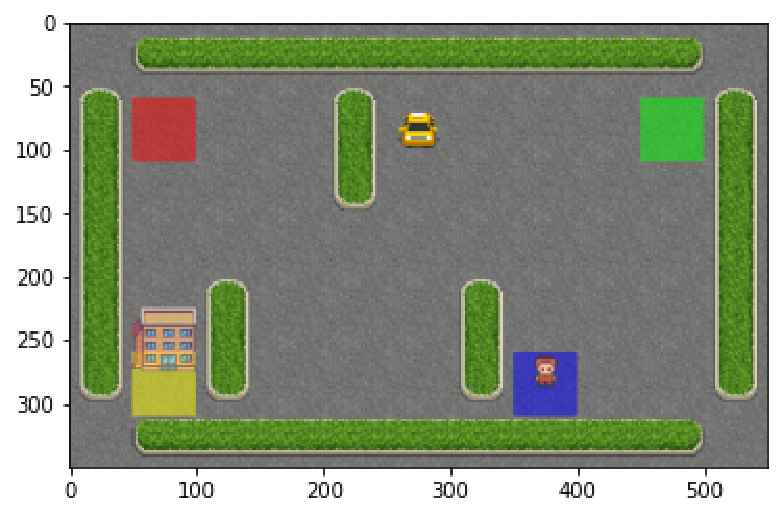
\includegraphics[width=10cm]{figures/taxi.pdf}
    \caption{Example starting position of \li{"Taxi-v3"}}
    \label{fig:taxi}
\end{figure}

\subsubsection*{SARSA(0)}
The main idea behind \emph{SARSA(0)}, or just \emph{SARSA}, is similar to Q-learning in that it approximates the optimal action-value function $q_*(s,a)$ using a Q-table.
The difference between SARSA and Q-learning is that SARSA uses the quality of the next state-action pair to update the value of the current state-action pair, whereas Q-learning uses the maximum quality available in the state-action pairs of the next state to update the value of the current state-action pair.
Thus, the equation for SARSA is given by
\begin{align}
    Q_{\text{new}}(s_t,a_t) &= Q_{\text{old}}(s_t,a_t) + \alpha\left[r_{t} + \gamma Q_{\text{old}}(s_{t+1},a_{t+1}) - Q_{\text{old}}(s_t,a_t)\right] \label{eq:sarsa_0} \\
                            &= (1-\alpha)Q_{\text{old}}(s_t,a_t) + \alpha\left[r_{t} + \gamma Q_{\text{old}}(s_{t+1},a_{t+1})\right] \nonumber,
\end{align}
where $r_{t} + \gamma Q_{\text{old}}(s_{t+1},a_{t+1})$ is the TD-target and the expression in the brackets of Equation\ \ref{eq:sarsa_0} (not the second equation below) is the TD-error.
Thus, the agent estimates the value of the current state-action pair by receiving the reward of the current state-action pair and then calculating an estimate of the value next state-action pair.
This is where the name SARSA comes from as the agent uses the quintuple $(s_t,a_t,r_t,s_{t+1},a_{t+1})$ to update the value of the current state-action pair using estimates of the next state-action pair.

The following pseudocode and the code block of Q-learning will help you implement the SARSA(0) algorithm.
Arrows with the tail end having the word \li{fill} signify that the given variable is assigned a value that you must fill in.
We give you some variables that may be harder to understand from just reading the \li{qlearn()} codeblock.

\begin{algorithm}[H]
\begin{algorithmic}[1]
    \Procedure{sarsa0}{env, alpha$=0.1$, gamma$=0.6$, epsilon$=0.1$, N$=70\_000$, decay$=$False}
        \State env$\gets$fill \Comment Make gym env
        \State sarsa\_tab$\gets$fill  \Comment Initialize Q-table (given by SARSA)
        \For{i in range(1,N+1)} \Comment Train

            \If{not decay}  \Comment Get epsilon value
                \State epsilon$\gets$epsilon
            \Else
                \State epsilon$\gets$epsilon\_decay(i, N)
            \EndIf

            \State curr\_s, info$\gets$fill \Comment Reset env and get current state s
            \State penalties, reward, done$\gets$fill  \Comment Initialize penalties, reward, done

            \If{random.uniform(0,1) $<$ epsilon} \Comment Get current action using epsilon-greedy algo
                \State curr\_act$\gets$fill
            \Else
                \State curr\_act$\gets$fill
            \EndIf

            \While{not done}
                \State next\_s, reward, done, trunc, info$\gets$fill \Comment Take current action, get new state, and reward

                \If{random.uniform(0,1) $<$ epsilon} \Comment Get next action using epsilon-greedy algo
                    \State next\_act$\gets$fill
                \Else
                    \State next\_act$\gets$fill
                \EndIf

                \State old\_val$\gets$fill \Comment Get the value of the current state and action
                \State next\_val$\gets$sarsa\_tab[next\_s, next\_act] \Comment Get the value of the next state and action\
                \State new\_val$\gets$fill \Comment Calculate the new value of the current state and action
                \State sarsa\_tab[curr\_s, curr\_act]$\gets$new\_val \Comment Update the Q-table

                \If{reward $==$ -10} \Comment Check for penalty according to Taxi env
                    \State penalties$+=1$
                \EndIf

                \State curr\_s$\gets$next\_s \Comment Update the current state
                \State curr\_act$\gets$next\_act \Comment Update the current action

            \EndWhile

        \EndFor
        \State env.close()
        \State \Return sarsa\_tab, penalties

    \EndProcedure

\end{algorithmic}
\caption{SARSA(0) Algorithm}
\label{alg:sarsa0}
\end{algorithm}

Before concluding the lab and moving on to the last problem, do note that both Q-learning and SARSA(0) can suffer from what is called \emph{maximization bias}.
However, we leave this off to the Additionals Materials section as it necessitates another topic we briefly touch on in the conclusion.
We strongly recommend reading this section to help you know potential problems with Q-learning and SARSA(0) and how to fix them when employing these algorithms in practice.

\section*{Wrapping Up}
The type of reinforcement learning we have worked with in Q-learning is called \emph{off-policy learning}.
This is a very important concept in RL, but we save it to the Additional Materials section were we discuss it in more detail along \emph{on-policy learning}, SARSA being an example.
This will help us understand the difference between the two types of learning and why we use them in different scenarios.
We strongly recommend reading this section to understand the difference between off-policy and on-policy learning.

Moreover, we have worked with \emph{online} reinforcement learning, where the agent learns from the environment in real-time.
That is, the agent interacts with the environment and learns from the environment as it goes, so it can keep gathering data as it continues to interact.
This is in contrast to \emph{offline} reinforcement learning, where the agent learns from a dataset of experiences that someone has collected from the environment so that the agent does not interact with the environment in real-time and cannot gather anymore data than the one given.

Lastly, this whole process of running the algorithm for $N$ episodes is what in machine learning is called \emph{training} the model.
Training the model is the process of feeding the model data and allowing it to learn from that data.
The objective of training is to learn the proper model parameters that will allow it to increase its performance in the given task.
In our case for model-free RL, training the model has the objective of exploring and exploiting the environment to learn the optimal policy.

\begin{problem}
\label{prob:sarsa}
    You will perform the following and use the \li{"Taxi-v3"} environment for the following problem:
    \begin{enumerate}
        \item Implement the \li{sarsa0()} function as given in Algorithm\ \ref{alg:sarsa0}.
        You will need\ \ref{eq:sarsa_0} to help you calculate the new value of the current state-action pair as well as the given code block of Q-learning to help you implement the function.
        You do not need to have a section that prints out the episode number or the completion of training as in the Q-learning function, but you can if you want.
        Do make sure to close the environment at the end of the function.
        We have already given you the penalty check for the Taxi environment.

        \item Then, use \li{sarsa0()} to calculate the optimal Q-table of the environment using the default values for the hyperparameters as given and the given default value for \li{N}.
        Employ a decaying epsilon value to calculate the Q-table.
        Render \li{"Taxi-v3"}, use the Q-table to move through it for one episode, and print the total reward.
        You will want to store this Q-table in a separate variable.
        The training time for the default N should be about the same as the training time for the Q-learning function with a decaying epsilon value.

        \item Finally, write a function \li{compare()} which initializes the \li{"Taxi-v3"} environment (without rendering).
        This function will compare the average total reward of 1000 episodes of the Q-learning and SARSA(0) tables that were created using a decaying epsilon.
        Run scenarios the Taxi environment for $1000$ episodes for each method using the tables you have now created.
        Return the average total reward for 1000 episodes for each algorithm.
        This is a tuple of two floats.
    \end{enumerate}

\end{problem}

\section*{Additional Materials}
\subsection*{More on the Epsilon-Greedy Algorithm}
We talked about the difficulty of the trade-off between exploration and exploitation and how using the $\epsilon$-greedy algorithm can help with this.
Using the epsilon-greedy algorithm is a simple way to balance the trade-off between exploration and exploitation, but it is not the only way.
Thompson sampling (taught in Volume 2 Chapter 17), Upper confidence bound (UCB), and Softmax Action Selection are other exploring strategies that can be used to handle the exploration-exploitation trade-off.
\cite{sutton2018reinforcement} makes a brief mention of these strategies, but they are not covered in depth.
However, there are plenty of free articles and blogs that cover these strategies in depth.

Rather than limiting ourselves to a constant epsilon value or a linear decay, we can use an exponential decay for $\epsilon$.
Using $\epsilon_1$ as the starting value of epsilon and $\epsilon_N$ as the ending value of epsilon, we can define the epsilon value for each episode $i\in\{1,\ldots,N\}$ as $\epsilon_1 * \lambda, \lambda=(\frac{\epsilon_N}{\epsilon_1})^{\frac{i}{N}}$.
We could multiply the episode $i$ in the numerator\footnote{There is no uniqueness of using $\beta$ in the numerator as the same effect can be had by using it in the numerator.} of $\lambda$ by $\beta$ to control the steepness of the decay, but be careful as this can affect the value for $\epsilon_N$.

\begin{problem}
    Update the function \li{epsilon_decay()} as given in problem 5 to now include in the parameters a string \li{decay_type} that defaults to \li{"linear"} that allows the user to choose between a linear and exponential decay.
    Use \li{"exp"} for exponential decay.
    Then, update the \li{qlearn()} function or \li{sarsa0()} function (below) to also include the same parameter \li{decay_type}.
    Test the function with both linear and exponential decay.
    You could also try other exploration strategies like Thompson sampling, UCB, and Softmax Action Selection and compare them to the \li{epsilon_decay()} function.
\end{problem}

\subsection*{Expected SARSA}
We give a full definition of the policy $\pi$ in the next lab.
For now, to be more detailed, $\pi$ takes in a state $s$ and returns a probability of taking an action $a\in A_s$.

Like Q-learning and SARSA(0), \emph{Expected SARSA} is a model-free reinforcement learning algorithm that approximates the optimal action-value function $q_*(s,a)$.
Specifically, Expected SARSA uses the expected value of the next state-action pairs to update the value of the current state-action pair.
That is, we take into account how likely we are to take a certain action in the next state under the current policy and use that to update the value of the current state-action pair.
Thus, we move in the direction of the expectation of the next state-action pairs (hence the name Expected SARSA).

The formula for Expected SARSA is given by
\begin{align*}
    Q_{\text{new}}(s_t,a_t) &= Q_{\text{old}}(s_t,a_t) + \alpha \Biggr[r_t + \gamma \mathbb{E}\bigr[Q_{\text{old}}(s_{t+1},a_{t+1}) \bigl\lvert s_{t+1} \bigl] - Q_{\text{old}}(s_t,a_t)\Biggl] \\
                            & = Q_{\text{old}}(s_t,a_t) + \alpha \Biggr[r_t + \gamma \sum_{a\in A_{s_{t+1}}} \pi(a|s_{t+1}) Q(s_{t+1},a)   - Q_{\text{old}}(s_t,a_t)\Biggl].
\end{align*}
In the case of a deterministic policy, the expected value of the next state-action pairs is the same as before.
When we do have a stochastic policy, we can use list comprehension to calculate the expected value of the next state-action pairs.
Note that Expected SARSA is an on-policy algorithm like SARSA.
We leave to the reader to determine which is the TD-target and the TD-error in the above equation.

\subsection*{Q-learning vs. SARSA vs. Expected SARSA}
Both Q-learning and SARSA are model-free reinforcement learning algorithms that approximate the optimal action-value function.
One of the main differences is that Q-learning uses the maximum quality of the next state-action pair to update the value of the current state-action pair, whereas SARSA uses the quality of the next state-action pair to update the value of the current state-action pair.
Thus, since Q-learning uses the best possible next action, it generally converges to the optimal policy faster than SARSA because SARSA could still take an exploratory action.
Moreover, SARSA typically tends to lead to more stable solutions than Q-learning as well yielding better cumulative rewards.
Both are great model-free algorithms to use.

SARSA gets the next action stochastically by, at least in our code, using the epsilon-greedy policy.
This creates variance in our estimates of the value of the state-action pairs.
While Expected SARSA is computationally more expensive than SARSA, it is more stable and can yield better cumulative rewards since it eliminates the variance found in SARSA.
However, this is occurs when the policy is highly stochastic.
In most cases, Expected SARSA is only slightly better than SARSA.

To implement this algorithm, employ the same pseudocode as given in Algorithm\ \ref{alg:sarsa0} and the given code block of Q-learning.
Then just replace the equation for the new value of the current state-action pair with the Expected SARSA equation using list comprehension to calculate the expected value of the next state-action pairs.
You will need to add in the parameter \li{policy} to the function to be able to obtain the probability of taking an action in the next state under the current policy.

\subsection*{On-Policy vs. Off-Policy Learning}
In model-free reinforcement learning, there are two types of learning: \emph{on-policy learning} and \emph{off-policy learning}.
The policy that the agent uses to determine its action/behavior as a response to its environment is called the \emph{behavior policy}.
Whereas, the policy that the agent uses to learn from the rewards of the actions taken and becomes the optimal policy is called the \emph{target policy} (i.e.\ the policy used to update the qualities/values of state-action pairs).
In \emph{on-policy learning}, the behavior policy and the target policy are the same or similar.
Whereas, in \emph{off-policy learning}, the behavior policy and the target policy are different.

The ultimate goal is to learn the optimal policy, denoted $\pi_*$, but the way we learn $\pi_*$ can be different.
In on-policy learning, the agent uses a common behavior and target policy to respond to the environment and then learn from the rewards of the actions taken in order to optimize the current values of the state-action pairs so that they converge to the optimal ones.
SARSA is an example of an on-policy learning algorithm.
In the TD-target expression of Equation\ \ref{eq:sarsa_0}, the policy used to take actions in the environment is similar to the policy used to update the value of the state-action pairs.
In our case, we used the epsilon-greedy algorithm/policy to determine the current action and the next action.
Even if we used a different method for how to choose an action, say UCB or Thompson sampling, the policy used to take actions in the environment would still be the same as the policy used to update the value of the state-action pairs.
You cannot use a different policy to take actions in the environment than the one you use to update the value of the state-action pairs because that will change the nature of SARSA so that it may not converge to the optimal policy.

Comparing this to Q-learning, an off-policy learning algorithm, the behavior policy and the target policy are different.
In this type of learning, the agent uses the behavior policy to take actions and then uses the target policy to update the value of the state-action pairs so that it converges to $\pi_*$.
In the TD-target expression of Equation\ \ref{eq:q_learning}, the policy the agent uses to explore or take actions in the environment, at least in our code, is the epsilon-greedy policy, but the policy the agent uses to update the value of the state-action pairs always chooses the action that maximizes the value of the next state-action pairs.
Thus, regardless of whatever the behavior policy tells us to do (i.e.\ explore or exploit according to the epsilon-greedy algorithm), the target policy will always choose the best action to update the value of the state-action pairs.
Hence, we have two different policies.

Overall, on-policy learning is a type of learning where the agent uses the same policy to take actions in the environment and to then update its estimates of a value function that will converge to the optimal value function.
In contrast, off-policy learning is a type of learning where the agent uses a one policy to take actions in the environment and another policy to then update its estimates of a value function that will go to the optimal value function.

\subsection*{Maximization Bias \& Double Q-Learning}
This section is a direct connection to the previous section comparing and contrasting Q-learning, Expected SARSA, and SARSA(0).
But we first had to introduce the vocabulary of on-policy and off-policy learning to understand the bias that can occur in both.

All of the given model-free methods involve maximization in the construction of their target policies.
There would be no problem if we did not have to approximate the value of the state-action pairs using other estimates of the value of the state-action pairs.
But the fact that we do, it leads to overestimation of the value of the state-action pairs as we take the maximum value.
It is the choice of estimator, the maximum value, that leads to the overestimation of the value of the current state-action pair since it is tied to its own value.
That is, we are using an estimate of the value of the next state-action pair to get an estimate of its maximum value over all possible actions in the action space to update the value of the current state-action pair.
Thus, we are using the same sample to both determine the maximizing action and to estimate its value.

One way to mitigate the maximization bias is to use \emph{Double Q-learning}.
Double Q-learning is an improvement to the normal Q-learning ideas of SARSA(0), Expected SARSA, and Q-learning.
The main idea is that rather than using the same sample to determine the maximizing action and to estimate its value, we use two different samples to determine the maximizing action and to estimate its value.
This can be applied to Q-learning, SARSA(0), and Expected SARSA, but we will only talk about implementing this idea in Q-learning.
The reader should be able to implement this idea in SARSA(0) and Expected SARSA as well.

The process of Double Q-learning is simple.
We take two Q-tables, $Q_1$ and $Q_2$, and use one to determine the maximizing action and the other to estimate its value.
We can use, for example, $Q_1$ to determine the maximizing action $a_*=\underset{a\in A_{s_{t+1}}}{\argmax}\text{ } Q_1(s_{t+1},a)$ and then use $Q_2$ to estimate its value $Q_2(s_{t+1},a_*)$.
We can then update the value of the current state-action pair using the following formula:
\begin{align*}
    Q_1(s_t,a_t) &= Q_1(s_t,a_t) + \alpha\left[r_{t} + \gamma Q_2(s_{t+1},\underset{a\in A_{s_{t+1}}}{\argmax} \{Q_1(s_{t+1},a)\}) - Q_1(s_t,a_t)\right] \\
                 &= Q_1(s_t,a_t) + \alpha\left[r_{t} + \gamma Q_2(s_{t+1},a_*) - Q_1(s_t,a_t)\right].
    \label{eq:double_q}
\end{align*}
This role can be reversed where we use $Q_2$ to determine the maximizing action and $Q_1$ to estimate its value.

For implementation, we can divide the alternating between the two Q-tables by a random number generator that chooses between the two Q-tables by simulating a coin flip (i.e.\ a 50-50 chance).
This way, we can alternate between the two Q-tables to determine the maximizing action and to estimate its value.
There is nothing special about the 50-50 chance, but it is a simple way to alternate between the two Q-tables.
Moreover, we can have the behavioral policy utilize the two Q-tables or just one of them.
If using two, we can use an average of the two or a sum.
Again, there is nothing special about the average or sum, but it is a simple way to combine the two Q-tables.
We can implement as follows (note we chose an action over the sum of the two Q-tables):
\begin{algorithm}[H]
\begin{algorithmic}[1]
    \Procedure{DoubleQLearn}{env, alpha$=0.1$, gamma$=0.6$, epsilon$=0.1$, N$=70\_000$, decay$=$False}
        \State env$\gets$gym.make(env)
        \State q1$\gets$ np.zeros((env.observation\_space.n,env.action\_space.n))  \Comment Initialize Q-tables
        \State q2$\gets$ np.zeros((env.observation\_space.n,env.action\_space.n))

        \For{i in range(1,N+1)} \Comment Train
            \If{not decay}  \Comment Get epsilon value
                \State epsilon$\gets$epsilon
            \Else
                \State epsilon$\gets$epsilon\_decay(i, N)
            \EndIf

            \State curr\_state, info$\gets$env.reset()  \Comment Reset env and get current state
            \State done$\gets$False
        
            \While{not done}
                \If{random.uniform(0,1) $<$ epsilon} \Comment Get current action using epsilon-greedy algo
                    \State curr\_action$\gets$env.action\_space.sample()
                \Else
                    \State curr\_action$\gets$(q1[curr\_state]+q2[curr\_state]).argmax()
                \EndIf

                \State next\_state, reward, done, trunc, info$\gets$env.step(curr\_action)

                \If{random.uniform(0,1) $< 0.5$} \Comment Update q1
                    \State max\_act$\gets$(q1[next\_state]).argmax()
                    \State qval$\gets$q1[curr\_state,curr\_action]
                    \State next\_qval$\gets$q2[next\_state,max\_act]
                    \State q1[curr\_state,curr\_action]$\gets$qval+alpha*(reward+gamma*next\_qval-qval)

                \Else \Comment Update q2
                    \State max\_act$\gets$(q2[next\_state]).argmax()
                    \State qval$\gets$q1[curr\_state,curr\_action]
                    \State next\_qval$\gets$q1[next\_state,max\_act]
                    \State q2[curr\_state,curr\_action]$\gets$qval+alpha*(reward+gamma*next\_qval-qval)

                \EndIf

                \State curr\_state$\gets$next\_state
            
            \EndWhile

        \EndFor

        \State \Return q1, q2
    \EndProcedure

\end{algorithmic}
\caption{DoubleQ Learning Algorithm}
\label{alg:double_q}
\end{algorithm}

This double Q-learning algorithm is a great way to mitigate the maximization bias that can occur in Q-learning, SARSA(0), and Expected SARSA.
The above given algorithm can be modified to work with SARSA(0) and Expected SARSA as well.
Note this does increase the spatial complexity of the algorithm as we now have two Q-tables to keep track of.
But, we are only using one Q-table to determine the maximizing action and the other to estimate its value so that temporal complexity is not affected.
While we have mitigated the maximization bias, it can be shown double Q-learning can lead to underestimation of the value of the state-action pairs.
But, this at least is better than overestimation.